\documentclass[11pt]{article}
\usepackage[top=2cm,bottom=2cm,left=2cm,right= 2cm]{geometry}
%\geometry{landscape}                % Activate for for rotated page geometry
\usepackage[parfill]{parskip}    % Activate to begin paragraphs with an empty line rather than an indent
\usepackage{graphicx}
\usepackage{amssymb}
\usepackage{epstopdf}
\usepackage{setspace}            
\usepackage{amsmath}            
\usepackage{multirow}    
\usepackage{changepage}
\usepackage{lscape}
\usepackage{ulem}
\usepackage{multicol}
\usepackage{dashrule}
\usepackage[usenames,dvipsnames]{color}       
\usepackage{enumitem}
\newcommand{\urlwofont}[1]{\urlstyle{same}\url{#1}}
\newcommand{\degree}{\ensuremath{^\circ}}

\DeclareGraphicsRule{.tif}{png}{.png}{`convert #1 `dirname #1`/`basename #1 .tif`.png}

\newenvironment{choices}{
\begin{enumerate}[(a)]
}{\end{enumerate}}

\thispagestyle{empty}

%\newcommand{\soln}[1]{\textcolor{MidnightBlue}{\textit{#1}}}	% delete #1 to get rid of solutions for handouts
\newcommand{\soln}[1]{ \vspace{2.7cm} }

\newcommand{\solnMult}[1]{\textbf{\textcolor{MidnightBlue}{\textit{#1}}}}	% uncomment for solutions
%\newcommand{\solnMult}[1]{ #1 }	% uncomment for handouts

%\newcommand{\pts}[1]{ \textbf{{\footnotesize \textcolor{black}{(#1)}}} }	% uncomment for handouts
\newcommand{\pts}[1]{ \textbf{{\footnotesize \textcolor{red}{(#1)}}} }	% uncomment for handouts

\newcommand{\note}[1]{ \textbf{\textcolor{red}{[#1]}} }	% uncomment for handouts

\definecolor{oiG}{rgb}{.298,.447,.114}
\definecolor{oiB}{rgb}{.337,.608,.741}

\usepackage[colorlinks=false,pdfborder={0 0 0},urlcolor= oiG,colorlinks=true,linkcolor= oiG, citecolor= oiG,backref=true]{hyperref}

%\usepackage{draftwatermark}
%\SetWatermarkScale{4}

\usepackage{titlesec}
\titleformat{\section}
{\color{oiB}\normalfont\Large\bfseries}
{\color{oiB}\thesection}{1em}{}
\titleformat{\subsection}
{\color{oiB}\normalfont}
{\color{oiB}\thesubsection}{1em}{}

\newcommand{\ttl}[1]{ \textsc{{\LARGE \textbf{{\color{oiB} #1} } }}}

\newcommand{\tl}[1]{ \textsc{{\large \textbf{{\color{oiB} #1} } }}}

\begin{document}

Dr. \c{C}etinkaya-Rundel \hfill Data Analysis and Statistical Inference \\

\ttl{Application exercise: 7.1 \\
Multiple linear regression}

\section*{Cigarettes and CO}

The Federal Trade Commission annually rates varieties of domestic cigarettes according to their tar, nicotine, and carbon monoxide content. The United States Surgeon General considers each of these substances hazardous to a smoker's health. Past studies have shown that increases in the tar and nicotine content of a cigarette are accompanied by an increase in the carbon monoxide emitted from the cigarette smoke.

In this exercise we will work with data from 2007 on cigarettes sold in the US. Each row in the dataset represents a cigarette. There are 11 variables in the dataset:
{\small
\begin{itemize}
\item \texttt{BRAND\_NAME}
\item \texttt{TYPE}: Type of cigarette, REGULAR or MENTHOL
\item \texttt{NIC}: Nicotine content, in mg
\item \texttt{TAR}: Tar content, in mg
\item \texttt{CO}: Carbon monoxide, in mg
\item \texttt{LEN}: Length of cigarette, in mm
\item \texttt{FLTR}: Filter, F or NF
\item \texttt{PACK}: Pack type, HARD or SOFT   
\item \texttt{STRENGTH}: Strength of cigarette, ULTRA LIGHT, LIGHT, MEDIUM, REGULAR FULL, or FLAVOR
\item \texttt{STYLE}: Some information of style of cigarette (not available for all cigarettes, and not used in this analysis)
\item \texttt{OTHER}: Other relevant information (not available for all cigarettes, and not used in this analysis)
\end{itemize}
}
To load the data use the following:
\begin{verbatim}
download("http://stat.duke.edu/~mc301/data/cig07.RData", destfile = "cig07.RData")
load("cig07.RData")
\end{verbatim}

\begin{enumerate}
\item First we try a full model with all explanatory variables in the model. The output of this model is shown below. Interpret the slopes of nicotine and tar variables. Are these results surprising? Why, or why not? Make sure to use appropriate terminology in your answer, and use summary statistics and/or visualizations of the data to support your answer.
{\small
\begin{center}
\begin{tabular}{rrrrr}
  \hline
 & Estimate & Std. Error & t value & Pr($>$$|$t$|$) \\ 
  \hline
(Intercept) & -0.5581 & 0.5406 & -1.03 & 0.3021 \\ 
  NIC & -4.0506 & 0.4357 & -9.30 & 0.0000 \\ 
  TAR & 1.0492 & 0.0441 & 23.77 & 0.0000 \\ 
  LEN & 0.0352 & 0.0055 & 6.37 & 0.0000 \\ 
  FLTRNF & -6.5050 & 0.3603 & -18.06 & 0.0000 \\ 
  PACKSOFT & 0.5130 & 0.1047 & 4.90 & 0.0000 \\ 
  STRENGTHLIGHT & 1.6867 & 0.2121 & 7.95 & 0.0000 \\ 
  STRENGTHMEDIUM & 0.7418 & 0.4616 & 1.61 & 0.1083 \\ 
  STRENGTHREGULAR & 0.2880 & 0.3072 & 0.94 & 0.3487 \\ 
  STRENGTHFULL FLAVOR & 2.2496 & 0.3292 & 6.83 & 0.0000 \\ 
  TYPEMENTHOL & -0.0332 & 0.1109 & -0.30 & 0.7647 \\ 
   \hline
\end{tabular}
\end{center}
}
\item Next, we try the following two models, and obtain the following adjusted $R^2$ values:
\begin{itemize}
\item Option 1, use TAR: \texttt{lm(CO $\sim$ TAR + LEN + FLTR + PACK + STRENGTH + TYPE, data = cig07)}, \\
adjusted $R^2$ = 0.7855
\item Option 2, use NIC: \texttt{lm(CO $\sim$ NIC + LEN + FLTR + PACK + STRENGTH + TYPE, data = cig07)}, \\
adjusted $R^2$ = 0.7066
\end{itemize}
Based on these results which variable should we keep in our full model, NIC or TAR? Why?

\item Suppose the final model (based on backwards p-value based elimination) as follows. Interpret the slope estimates associated with the strength variable. Based on this model, cigarettes with which strength level has the highest CO emissions?

{\small
\begin{center}
\begin{tabular}{rrrrr}
  \hline
 & Estimate & Std. Error & t value & Pr($>$$|$t$|$) \\ 
  \hline
(Intercept) & -0.0586 & 0.5555 & -0.11 & 0.9160 \\ 
  TAR & 0.7344 & 0.0293 & 25.07 & 0.0000 \\ 
  LEN & 0.0267 & 0.0056 & 4.76 & 0.0000 \\ 
  FLTRNF & -6.1949 & 0.3686 & -16.81 & 0.0000 \\ 
  PACKSOFT & 0.5597 & 0.1081 & 5.18 & 0.0000 \\ 
  STRENGTHLIGHT & 1.9077 & 0.2168 & 8.80 & 0.0000 \\ 
  STRENGTHMEDIUM & 0.7900 & 0.4766 & 1.66 & 0.0976 \\ 
  STRENGTHREGULAR & 0.5664 & 0.3149 & 1.80 & 0.0723 \\ 
  STRENGTHFULL FLAVOR & 3.0920 & 0.3268 & 9.46 & 0.0000 \\ 
   \hline
\end{tabular}
$:$ \\
Multiple R-squared:  \textcolor{oiB}{[$R^2$]},	Adjusted R-squared:  \textcolor{oiB}{[$R^2_{adj}$]} \\
F-statistic: \textcolor{oiB}{[$F$]} on \textcolor{oiB}{[$df_1$]} and \textcolor{oiB}{[$df_2$]} DF,  p-value: $<$ 2.2e-16
\end{center}
}

\item Use the following plots to check conditions for this model.

\end{enumerate}

\begin{center}
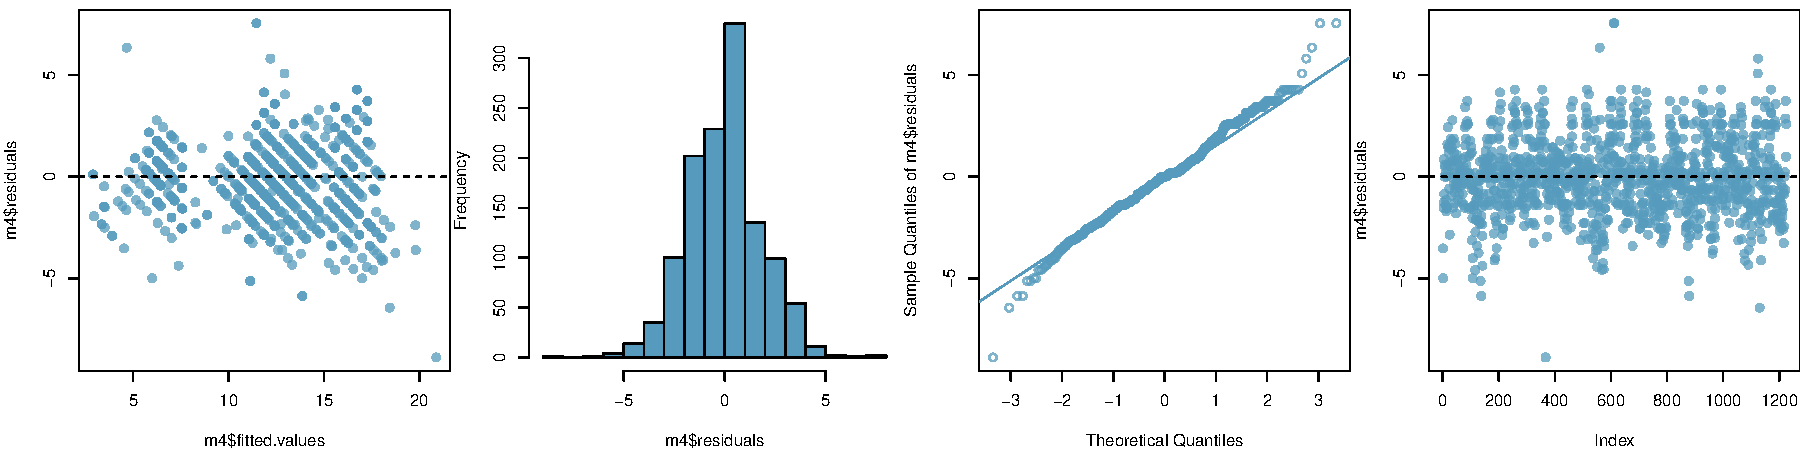
\includegraphics[width=\textwidth]{diag.pdf}
\end{center}

\begin{enumerate}[resume]

\item Construct a 95\% confidence interval for the slope of the filter variable (FLTRNF), and interpret it in context.

\item Using the ANOVA output for the model provided below, calculate the \textcolor{oiB}{\textit{[redacted]}} statistics on the regression output above. \textit{Hint:} The ANOVA output below shows SS attributed to each variable separately, $SS_{Regression}$ is the sum of those.

\begin{center}
\begin{tabular}{lrrrrr}
  \hline
 & Df & Sum Sq & Mean Sq & F value & Pr($>$F) \\ 
  \hline
TAR & 1 & 12216.31 & 12216.31 & 3622.74 & 0.0000 \\ 
  LEN & 1 & 194.02 & 194.02 & 57.54 & 0.0000 \\ 
  FLTR & 1 & 1675.48 & 1675.48 & 496.86 & 0.0000 \\ 
  PACK & 1 & 169.17 & 169.17 & 50.17 & 0.0000 \\ 
  STRENGTH & 4 & 900.44 & 225.11 & 66.76 & 0.0000 \\ 
  Residuals & 1216 & 4100.50 & 3.37 &  &  \\ 
   \hline
\end{tabular}
\end{center}

\item In this model, which predictor is able to explain the highest portion of the variability in CO emission of cigarettes?

\item Using the regression model predict the CO emission for a cigarette with the following characteristics. Note that you may not need to use each attribute in your calculation.

\begin{multicols}{2}
\begin{itemize}
\item \texttt{BRAND\_NAME}: Sir Smokes-a-Lot
\item \texttt{TYPE}: MENTHOL
\item \texttt{NIC}: 0.75 mg
\item \texttt{TAR}: 12 mg
\item \texttt{LEN}: 80 mm
\item \texttt{FLTR}: F
\item \texttt{PACK}: HARD
\item \texttt{STRENGTH}: LIGHT
\end{itemize}
\end{multicols}

\item Now confirm your prediction from the previous question using the \texttt{predict} function in R. Note that your hand calculated prediction might be very slightly different from R's prediction, due to rounding of the coefficients on the regression output.
\begin{verbatim}
# fit the model
m = lm(CO ~ TAR + LEN + FLTR + PACK + STRENGTH, data = cig07)
# create the new data point
smokesalot = data.frame(TAR = 12, LEN = 80, FLTR = "F", PACK = "HARD", STRENGTH = "LIGHT")
# predict
predict(m, newdata = smokesalot)
\end{verbatim}

Include your R code and your write up in your submission. 

If you have questions about the R syntax, refer to \url{https://stat.duke.edu/~mc301/R/Rcommands.pdf} or ask.

 \end{enumerate}

%

\end{document}